% This is LLNCS.DOC the documentation file of
% the LaTeX macro package from Springer-Verlag
% for Lecture Notes in Computer Science, version 1.2
\documentclass[runningheads,a4paper]{llncs}
%
%\usepackage[numbers]{natbib}
\usepackage{hyperref}
\usepackage{amsmath}
\usepackage{dcolumn}
%\usepackage{endnotes}
\usepackage{graphics}
\usepackage{graphicx}
\usepackage{algorithm}
\usepackage{algorithmic}
%\para codigo de programación
\usepackage{listings}
%\usepackage{lineno,hyperref}

\newfont{\titelfont}{cmr10 scaled 1728}
\newfont{\titelbffont}{cmbx10 scaled 2074}
\newfont{\titelbigfont}{cmr10 scaled 2488}
\markboth{Style File for Authors Coding with \LaTeX{}}{Style File
for Authors Coding with \LaTeX{}}

\newtheorem{defn}{Definition}

%
\begin{document}
%
\title{An extension of PRONTO ontological model for Manufactured Physical Artifacts}

\author{Liudmila Reyes-Alvarez\inst{1}, Marcela Vegetti\inst{3}, Luis J. Rodr{\'i}guez-Mu{\~n}iz\inst{2} and Irene D{\'i}az\inst{1}}

\institute{Dept. of Computer Science. University of Oviedo,\\ Oviedo, Asturias, Spain,
\and
Dept. of Statistics and O.R. University of Oviedo,\\Oviedo, Asturias, Spain\\
\and
Instituto de Desarrollo y Dise{\~n}o - INGAR, CONICET - UTN\\ Santa Fe, Argentina}

\maketitle
%
\begin{abstract}
 Technological distribution companies focuses on selling Manufactured Physical Artifacts, which are technological systems composed by physical electromechanical artifacts optimally configured to solve a specific problem in certain environment. These companies, which act as intermediary between customers and suppliers, play an important role in the distribution chain of physical electromechanical artifacts in industry. New lines of technological physical artifacts have dramatically increased the number of products among which, the mentioned companies have to choose the component needed to build and configure the Manufactured Physical Artifacts they provide to customers. The greater the number of products in the artifact database, the harder the tasks of selecting and configuring the artifacts required to build the optimal solution for a customer. A proposal for an ontological model supporting representation and management of physical electromechanical artifacts is presented in this article. Our model is an extension of \textit{PRONTO (PRoduct ONTOlogy)}, which is an ontology for comprehensive and consistent representation of product information that can be specialized in specific product domains. Based on PRONTO and in the \textit{Bill of Materials (BOM)} concept, the proposal helps this kind of companies in the representation of physical electromechanical artifacts, the constraints among them and their optimal configuration.
\end{abstract}
%
\section{Introduction} 

Companies focused on product distribution need to reinvent their business due to Malls and e-commerce competence. Thus, they should provide a well fitted answer to each customer but at the same time, they should provide a solution faster than others. To sum up, they must offer something different to attract customers. With the amount of different basic products they manage plus new products they can offer using the basic ones, a modern information management is required in order to make seller's job easier and more efficient. 

The current time to mine product databases is unacceptable as customers not only need a precise answer (that means, a technological artifact satisfying their requirements) but also a fast answer. As consequence, workers in charge to provide the answer to customers don't explore all the available products and restrict their-selves to recommend artifacts (complex products) considering only few products. Thus, it is required an information model allowing them to speed up information retrieval process. This model is the basis to construct an agile decision support system to help in the configuration of efficient artifacts in the industry of technological artifacts. In this sense, the use of metadata and ontologies represents a solution \cite{berners2001semantic} as the structure and relations between artifacts can be stored and mined.

In the last few years, many software solutions\cite{hepp2006products}, \cite{hepp2008goodrelations}, \cite{stolz2014pcs2owl}, \cite{vegetti2011pronto}, \cite{Reyes-Alvarez:2016} have been developed based on ontologies as a retrieval and classification model of information about catalogs of product-service. These models allow to categorize the information in business sceneries by the meaning of words related to the sector in question. Applications can retrieve data according to the knowledge stored in these models following different strategies \cite{Reyes-Alvarez:2016}.

In fact, some ontology models have been used to define both product offers and to implement marketing strategies to transform company resources in \textit{Value} \cite{andersson2006towards}, \cite{pigneur2002ontology}, \cite{rese2013ontology}. 
Other possibility is to design models based on international standards. Many isolated solutions have been developed to enhance the information retrieval and search relating to an specific product-service (for example UNSPSC\footnote{United Nations Standard Products and Services Code(UNSPSC). https://www.unspsc.org/} or the RosettaNet standard\footnote{A consortium of major Computer and Consumer Electronics, Electronic Components, Semiconductor Manufacturing, Telecommunications and Logistics companies working to create and implement industry-wide, open e-business process standards. https://supplier.intel.com/static/B2Bi/RosettaNet.htm}). 

It is also possible to consider taxonomies as ontologies and define the meaning of terms related to a certain industry domain. Taxonomy is based on the need of managers to organize their contracts, invoices, reports and other documents, which should have a coherent organization for their further search \cite{wemmerlov1990taxonomy}, \cite{diaz1998semi}. A taxonomy simply requires its components to be organized in order to carry out a successful classification. However, the interpretation of the taxonomic relationship is an important modeled decision.  

Other choice is to develop ontological representations oriented to product description according to its form or composition. An efficient information retrieval with regard to a particular product through suppliers, commercial partners and customers is allowed in business scenarios if and only a well-defined conceptual design is available. Ontologies and metadata have been considered an optimal solution for a conceptual design of tools as basis of product-service description between a company and its partners. In addition, it is possible to represent the knowledge from a particular application domain, which goes beyond research-development projects because the handled ontological representations provide relevant information about product-service in a given area of the industry (\cite{vegetti2011pronto}, \cite{nederstigt2014floppies}). 

Finally, this research is an extension of \textit{PRONTO (PRoduct ONTOlogy)}\cite{vegetti2011pronto} which is a proposed ontological model for comprehensive and consistent representation of product information that can be specialized in specific product domains.
This ontology allows the representation of data for products at different levels of abstraction. They define an \textit{Abstraction Hierarchy} and an \textit{Structural Hierarchy}, each one with a different role in the ontological model. On the one hand, \textit{Abstraction Hierarchy} allows unstructured representation of information products at different levels of abstraction, and aggregated representation and disaggregation of information among these abstraction levels. On the other hand, \textit{Structural Hierarchy} contains information about the products and components involved in product manufacture. The model handles relations among product structures, but only through \textit{componentOf} and \textit{derivateOf} relations. One of the main advantages of this proposal is that it defines a representation for a \emph{Bill of Materials (BOM)} of products that are semi-manufactured by assembly of component parts, given its level of abstract hierarchy.  

On based on this proposal, we design a knowledge representation based on an ontology to describe technological artifacts based on a new BOM. However, an ontological model satisfying all needs for physical technological artifacts information retrieval in the industry is not easy to obtain. To the best of our knowledge, this work is a first attempt to propose an ontological model on the basis of a new BOM focused in a \emph{Bill of Parts (BOP)} from a new part concept abstraction for manufactured technological artifacts. This work describes the features of this new ontological model.

The ontological model proposes an extension of PRONTO based on adaptation of a \emph{Bill of Materials} (BOM) to the needs of this enterprise type in the industry of technological artifacts. Therefore, this work is organized as follows. Section \ref{PRONTO} introduces a preliminaries about PRONTO model. Section \ref{BOP} describes the features of an adaptation of BOM with the name of \emph{Bill of Parts} (BOP) to satisfy the needs of intermediary companies in the industry of technological artifacts. The BOP proposed is the basis to develop our ontology. Section \ref{BOP} describes the new ontological model. Finally, Section \ref{C} shows conclusions and future work.

\section{PRONTO Ontological Model} \label{PRONTO}
AQUÍ VA UNA DESCRIPCION GENERAL Y RESUMIDA DEL MODELO PRONTO. DE FORMA TAL QUE LOS REVISORES ENTIENDAN EL MODELO PRONTO.

\section{\emph{Bill of Parts} (BOP) from \emph{Bill of Materials} (BOM)} \label{BOP}

In this section part identification as well as relations established between parts in each configuration sequence are described. BOM models play an important role because a model is defined as \emph{an structured list of the parts used to obtain a product}\cite{levy1986bill}. The rise of new technologies lead to creation of some approaches of BOMs such as those proposed by \cite{hegge1991generic}, \cite{willis1996method}, \cite{stonebraker1996restructuring}, which present models to adapt the BOM to the different needs. 

The BOM model proposed here is defined as \emph{an structured list of the parts (physical artifacts) used to configure a technological artifact determined}. Thus, the materials are parts that have been previously manufactured. We will refer to "\emph{Bill of Parts (BOP)}" instead of BOM from now on, the reason is because in this type of companies, solutions are created from already manufactured parts which are not produced by the organization. BOP is a generative BOM\cite{hegge1991generic}$^,$ \cite{willis1996method}$^,$ \cite{stonebraker1996restructuring}. Generative BOMs do not store the structural configuration of each technological artifact in the representation model. In contrast, this structure is generated from a basic structure previously defined.

A BOP of previously manufactured physical artifacts is composed of the parts shown in Figure \ref{BPA}. Each one of these parts are described below.
\begin{figure}[h]
\centering
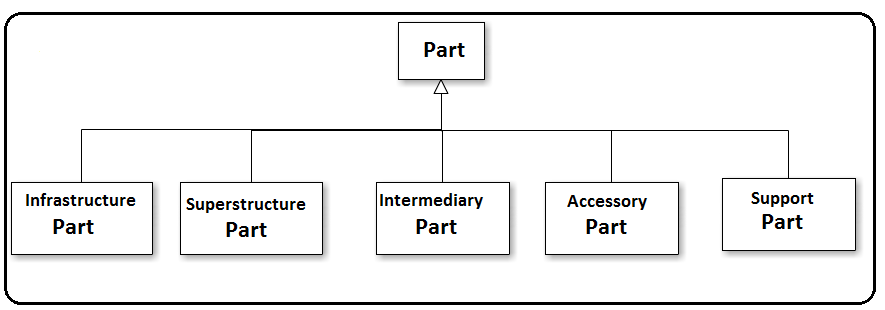
\includegraphics[scale=0.5]{Part2.png}
\caption{"\emph{Bill of Parts (BOP)}"}\label{BPA}
\end{figure}

\begin{itemize}
  \item \textbf{Infrastructure parts} are parts used as a basis for assisting the corresponding artifact (as a \textit{Whole}) and that interact with other similar parts.  
 \item \textbf{Superstructure parts} are parts employed as an interaction layer between external agents and infrastructure parts. Each artifact must contain at least one of each kind of these artifacts. For example, given an artifact that is a light switch system (see Figure \ref{TP}), intercom phones are a type of superstructure physical artifact, because at least one of them is required for the artifact (as a \textit{Whole}) to be functional.
\item \textbf{Intermediate parts} are those parts that connects other two parts of the artifact to configure. An important observation is that this type of part can be also an infrastructure or superstructure part. 
  \item \textbf{Accessory parts} are those parts used as a complement or ornament. These parts are not necessary for the correct performance of the artifact to configure. Besides, these parts are in physical contact with some of the other parts of the artifact. 
  \item \textbf{Support parts} are those parts that serve as support (or support the remaining parts of the artifact). Physical contact is established with all the parts that are held in it.
\end{itemize}

\begin{figure}[h]
\centering
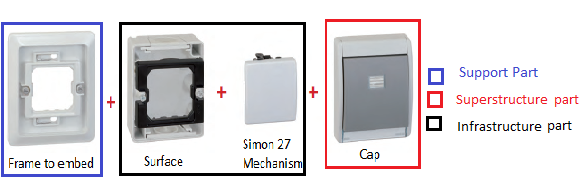
\includegraphics[scale=0.9]{TP.png}
\caption{Examples of technological artifacts: the part concept abstraction in a switch artifact for difficult environments.}\label{TP}
\end{figure}
Figures \ref{TP} and \ref{TP2} illustrates two examples of different technological artifacts where the parts that conform to it are identified: Figure \ref{TP} presents the part concept abstraction in a switch artifact for difficult environments and, Figure \ref{TP2} shows the part concept abstraction in an Hydraulic Mini-station.  
\begin{figure}[h]
\centering
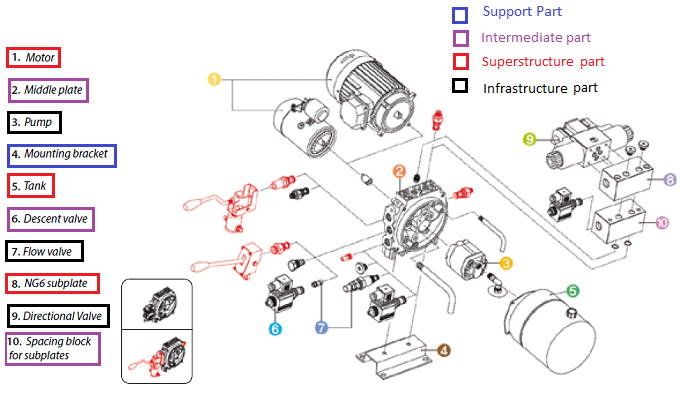
\includegraphics[scale=0.6]{E2.png}
\caption{Examples of technological artifacts: the part concept abstraction in an Hydraulics Mini-stations.}\label{TP2}
\end{figure}

Note that the different parts shown in Figure \ref{BPA} and describe previously are  classified according to the role they play within the artifact during configure process by installer or solutions creator. These definitions of parts describe the classes making up our ontological model. A technological artifact could not have within its compositional structure all the abstractions of the concept defined above, it can include from a single type to all abstraction types. For example if it has a part of each type of the abstraction concepts specified then the remaining parts will be placed on the support part. 

Furthermore, the superstructure part is to be connected to the infrastructure parts through the intermediate parts. In addition both superstructure and intermediate parts as well as the superstructure parts may have associated accessory parts. Also the superstructure part is where external agents, human beings, another devices (such as any physical artifact) or the environment interact.

\subsubsection{BOP Classification}
This subsection describes different classifications for BOPs. According to its compositional structure, BOPs can be classified as: 
\begin{itemize}
  \item \textbf{Atomic structure:} BOP composed by only a part which cannot be divided into other parts. That means the artifact is considered as a whole to design other more complex artifact. Some examples of this type of artifacts are a \emph{thermostat} or a heating system (for example: \emph{CPG-215M Saivod Split Wall Heater}). 
  \item \textbf{Non-atomic structure:} BOP with at least two different parts related to each other to form its structure. These parts are those described above which abstract the "\textbf{part}" concept (see figure \ref{BPA}). 
\end{itemize}

The above classification is necessary as basis to the ontological model because it is important to know whether an artifact must be represented as a combination of some parts or not. In addition, it is also important to know which artifacts have only a unique part. 
\begin{figure}[h]
\centering
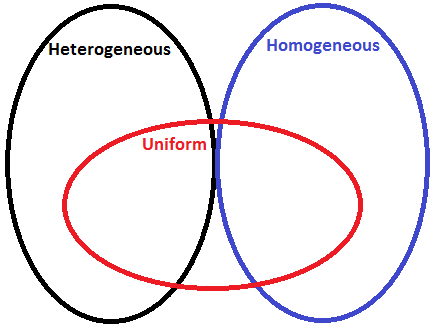
\includegraphics[scale=0.4]{Venn.png}
\caption{Artifact classification.}\label{Venn}
\end{figure}

On the other hand, BOPs are classified according to \emph{the diversity of parts and feature  parts} that compose the artifact. In this sense, the following classification is proposed:
\begin{itemize}
   \item \textbf{Heterogeneous structure:} An artifact whose parts are different one to each other due to the classes that define them or to the role within the artifact.
  This structure can have from $1$ to $n$ parts of different types related to each other.
   \item \textbf{Homogeneous structure:} An homogeneous BOP describes the same type of part based on a quantitative measure (example: a metre of cable). This structure can have from $1$ to $n$ parts of the same type related to each other.
  \item \textbf{Uniform structure:} An uniform BOP describes an artifact composed of parts that can be classified under an unique condition (a property, an attribute, etc.) This structure can be heterogeneous or homogeneous (see Figure \ref{Venn}).   
\end{itemize}

This classification with regard to structure gives us relevant information about whether an artifact is configured with same parts or different parts, or whether their configuration is governed by a specified condition or not. In addition, there all atomic structures are homogeneous while non-atomic ones can be heterogeneous, homogeneous or uniform (see figure \ref{CS}). 

\begin{figure}[H]
\centering
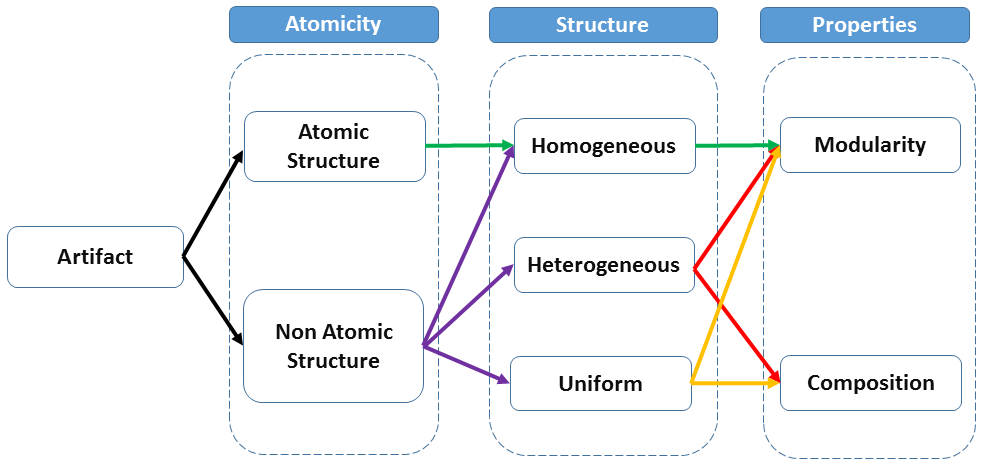
\includegraphics[scale=0.4]{SC2.png}
\caption{Classifications with regard to structure.}\label{CS}
\end{figure}

In addition, BOPs' structure presents the following properties.

\subsubsection{BOP Properties}
According to the specific domain requirements, BOP structures contain information about their composition and modularity. 
\begin{itemize}
\item \textbf{Composition}. It provides information about the compositional structure. 
\item \textbf{Modularity}. A BOP structure has a modular structure when it is possible to connect the artifact defined by this BOP structure to other artifact. Modularity property must establish the maximum number of connections that an artifact (or an artifact part) supports. 

For example: If an artifact as server system type has: 1) two power supplies (ie, two wires to plug into the mains); 2) four network cards (i.e four ports to connect to the network) and 3) a wifi connector, then it supports a maximum of seven connections (i.e. seven modules where only two modules are for power supplies, four modules are for connection to the wired network and a module is for connection to the wifi network). 
\end{itemize} 

\section{Extension of the PRONTO Ontological Model} \label{M}
The above defined BOP is the basis to develop an ontological model allowing the derivation of BOP structures that comply with the features described in previous sections.
\begin{figure}[H]
\centering
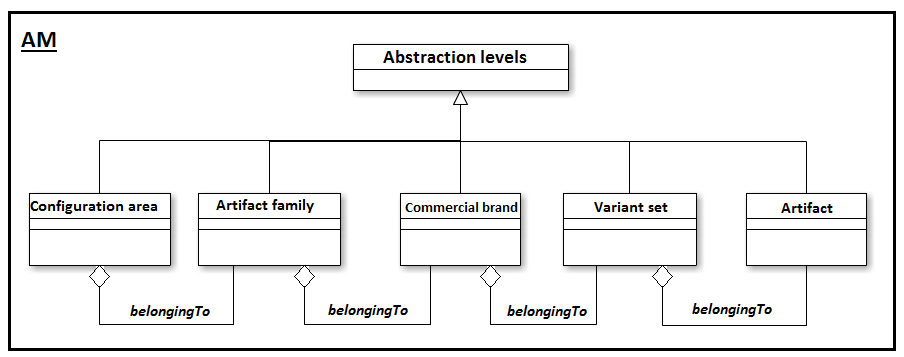
\includegraphics[scale=0.5]{AM.png}
\caption{Abstraction levels of the \textit{Abstraction Model}.}\label{AM}
\end{figure}

Like the ontology PRONTO\cite{vegetti2011pronto}, this extension describes an \textit{Abstraction Model (AM)} and a \textit{Structural Model (SM)}, each one with a different role. 

On one hand, unlike of PRONTO model, our proposed of AM allows an unstructured representation of information more detailed about physical electromechanical artifacts at different abstraction levels (see Figure \ref{AM}). These levels are defined as follows by our ontological model:
\begin{enumerate}
  \item \textbf{Configuration Area:} It represents the highest level of specification and defines the artifact set that respond to the same general functionality but with different behaviors. This level consists of at least one artifact family.
  \item \textbf{Artifact Family:} It represents the fourth level and defines the artifact set that have similar functionalities and behaviors but belongs to different commercial brands.
  \item \textbf{Commercial Brand:} It is the third level and defines the name or label that is assigned to an artifact set to distinguish it (or to denote quality or membership of a particular supplier).
  \item \textbf{Variant Set:} It is the second level and defines same artifact brand with similar functionalities and behaviors but with at least one characteristic that distinguishes them from the rest of artifacts of the same family.
  \item \textbf{Artifact:} It is the lowest level and represents individual items that are members of a particular variant set, so it has the structure associated with that set. This structure is constituted by other artifacts or physical parts.
\end{enumerate} 

These abstraction levels have the following properties:
\begin{itemize}
\item They are related through \emph{belongingTo} relationship (see Figure \ref{AM}) which will be one of the relationships of the ontological model. 
\item Each level of abstraction defines one of the classes of the ontological model.
\item All levels describe a uniform structure except the artifact level because these levels describe structures that will be grouped under the same condition. This implies that these levels may also include homogeneous or heterogeneous structures (see Figure \ref{Venn}). In the case of the artifact level, this may describe any of the three structure types (it depends on the parts that make up the artifact or the conditions that characterize it). 
\end{itemize}

On other hand, SM contains information about the parts (products or components) involved in an artifact configuration sequence. This is generated from the BOP in correspondence with the level of abstraction that is being referenced. With respect to the artifact level, the generated BOP describes each one of the types of structures defined in the previous section. With respect to other levels, the generated BOP describes uniform structures that inherit the structures of the artifacts which are members of that abstraction level. 

One of the main advantages of our proposal is that it defines a SM representation for any BOP of built artifacts given its level of AM. Each level of abstraction has one associated SM, i.e., each AM has one associated SM. In our case, the associated SM with the lowest level of abstraction (Artifact) is described in a more specific way because each SM of the remaining abstraction levels inherits the SM of the artifacts which belong to that level of abstraction. Therefore, belonging to a level of abstraction is provided by some restriction or modification (addition, delete) in the features or attributes of the artifact. Such restriction must be explicitly specified to distinguish a given set of artifacts.

\subsection{Structural Model (SM)}\label{HM}
Given that each AM has one associated SM, in this subsection, the structural model of our ontology is described. It enables the qualitative description of the relationships between the parts of the physical electromechanical artifact to configure by adding information related to their configuration sequence. 

The proposed \emph{SM} to configure physical electromechanical artifacts has two components:
\begin{enumerate}
\item \textbf{Part concept abstraction} define a BOP proposed by us. These are described in previusly sections.
\item \textbf{Part-Whole relationships} are defined on the base of the \textit{partOf} and \textit{connectedTo} relationships, the so called mereotopology. Note that mereotopology describes the relation that exists between the parts making up a whole (the relations between those parts) and their relation with the whole (the relation of the parts with the whole) \cite{smith1996mereotopology}$^,$\cite{varzi1993bbm}$^,$\cite{varzi1996parts}. These describe some of the Slots of our ontological model. 
\end{enumerate}

Mereotopology represents the union of a mereology and topology. Therefore, mereotopology is described from the \emph{partOf} (P) and \emph{connectedTo} (C) predicates.
The definitions and axioms that describe the Part-Whole relationships that can take place in the structures generated by \emph{SM} are
described in the following subsection. Basic definitions of the mereotopological primitives of interest for the proposed ontology are provided \cite{smith1996mereotopology} $^,$\cite{varzi1993bbm}$^,$ \cite{varzi1996parts}.

\subsubsection{Part-Whole relationships}\label{SH}
Definitions and axioms of the Part-Whole relationships allowed by \emph{SM} are described. Each relationship is defined by a predicate logic primitive ($R(x,y)$ describes a particular relation between two classes) The mereotopological primitives suitable for \emph{SM} are detailed in Tables \ref{tab:1} and \ref{tab:2}.% Give a unique label

According to Varzi\cite{varzi1993bbm}$^,$ \cite{varzi1996parts} and Smith\cite{smith1996mereotopology} who have studied in depth mereotopological primitives, both "x is part of y"(P(x,y)) and "x connected to y"(C(x,y)) are the starting points of these theories. Note that \textit{P} and \textit{C} must satisfy the following properties: 
\begin{itemize}

  \item \textit{part of} ($P$) must be \textit{reflective},  \textit{antsymmetric} and \textit{transitive}\cite{smith1996mereotopology}$^,$\cite{varzi1993bbm}$^,$\cite{varzi1996parts}.
  
\item \textit{connectedTo}($C$) is at least \textit{reflective} and \textit{symmetric}, \textit{monotonous with respect to \textit{partOf}} \cite{smith1996mereotopology}$^,$\cite{varzi1993bbm}$^,$\cite{varzi1996parts} which means that if an artifact is connected to a \textit{Part} is also connected to the \textit{Whole}.
\end{itemize}

\begin{table}
% table caption is above the table
\caption{Description of mereotopological primitives for Part-Whole relationships with a heterogeneous structure}
\label{tab:1}       % Give a unique label
% For LaTeX tables use
\begin{tabular}{ll}
\hline\noalign{\smallskip}
Mereotopological description  & Predicate \\
\noalign{\smallskip}\hline\noalign{\smallskip}
${PP}(x,y):={P}(x,y)\wedge\neg{P}(y,x)$ & `\textit{$x$ is proper part of $y$}' \\
\noalign{\smallskip}\hline\noalign{\smallskip}
${O}(x,y):=\exists{z}({P}(z,x)\wedge{P}(z,y))$ & `\textit{$x$ overlaps $y$}' \\
\noalign{\smallskip}\hline\noalign{\smallskip}
${U}(x,y):=\exists{z}({P}(x,z)\wedge{P}(y,z))$ & `\textit{$x$ underlaps $y$}' \\
\noalign{\smallskip}\hline\noalign{\smallskip}
${D}(x,y):={U}(x,y)\wedge\neg{O}(x,y)$ & `\textit{$x$ is discreet from $y$}' \\
\noalign{\smallskip}\hline\noalign{\smallskip}
${OX}(x,y):={O}(x,y)\wedge\neg{P}(x,y)$ & `\textit{$x$ over crossing $y$}' \\
\noalign{\smallskip}\hline\noalign{\smallskip}
${UX}(x,y):={U}(x,y)\wedge\neg{P}(y,x)$ & `\textit{$x$ under crossing $y$}' \\
\noalign{\smallskip}\hline\noalign{\smallskip}
${PO}(x,y):={OX}(x,y)\wedge{OX}(y,x)$ & `\textit{$x$ proper overlap $y$}' \\
\noalign{\smallskip}\hline\noalign{\smallskip}
${PU}(x,y):={UX}(x,y)\wedge{UX}(y,x)$ & `\textit{$x$ proper underlap $y$}' \\
\noalign{\smallskip}\hline\noalign{\smallskip}
${EC}(x,y) := {C}(x,y) \wedge \neg {O}(x,y)$ & `\textit{$x$ external connection $y$}' \\
\noalign{\smallskip}\hline\noalign{\smallskip}
${TP}(x,y) := {P}(x,y) \wedge \exists z ({EC}(z,x) \wedge {EC}(z,y))$ & `\textit{$x$ tangent part $y$}' \\
\noalign{\smallskip}\hline\noalign{\smallskip}
${IP}(x,y) := {P}(x,y) \wedge \neg {TP}(x,y)$ & `\textit{$x$ interior part $y$}' \\
\noalign{\smallskip}\hline\noalign{\smallskip}
${B}(x,y):=\forall{z}({P}(z,x) \rightarrow\forall{w}({IP}(z,w)$ & `\textit{$x$ boundary part $y$}' \\
$\rightarrow{O}(w,y)\wedge\neg{P}(w,y))$ & \\
\noalign{\smallskip}\hline
\end{tabular}
\end{table}

Tables \ref{tab:1} and \ref{tab:2} show the axioms defining the mereotopology associated to the proposed model. Firstly, the \emph{partOf} relation is described, where $P(x,y)$ means "\emph{x is part of y}", and it represent parthood for any artifact. Based on this primitive, other primitives can be further derived. Thus, the first derived is that "\emph{x is proper part of y}", denoted $PP(x,y)$, when if $x$ is part of $y$ then $y$ not is part of $x$. The second primitive is that "\emph{x overlaps y}", denoted $O(x,y)$, when $z$ is any part of $x$ and $y$. Besides the primitive "\emph{x underlaps y}" is derived too, denoted $U(x,y)$, when $x$ is part of any $z$ and also $y$ is part of $z$. All these definition are taken from \cite{varzi1996parts}. Another primitive is "\emph{x is discrete from y} ($D(x,y)$), which means that $x$ does not overlap $y$\cite{smith1996mereotopology}. This definition would be complete if "\emph{x underlap y}" is added because the relation $U(x,y)$ allows us to ensure that both parts belong to a common whole. The primitive "\emph{x is interior part of y}" is derived from P and denoted $IP(x,y)$ \cite{smith1996mereotopology}$^,$\cite{varzi1993bbm}$^,$\cite{varzi1996parts}. Other primitives that are derived from P are "\emph{x over crossing y}", "\emph{x under crossing y}", "\emph{x proper overlap y}", "\emph{x proper underlap y}"\cite{varzi1996parts} as well. Crossover relationships are important to represent cases where one artifact is over-cross by another or vice versa, for example an artifact which makes the protective cover of another overcrossing it. "\emph{x proper overlap y}", "\emph{x proper underlap y}" relationships are important to represent relationships such as those established between the shackles of a classic chain where both objects are over or under cross.

The following primitives are derived from $C(x,y)$ that means "\emph{x is connected to y}". Then it leads to the introduction of the primitives of: "\emph{x is boundary of y}" denoted $B(x,y)$, "\emph{x external connection y}" denoted $EC(x,y)$ and "\emph{x part tangent y}" denoted $TP(x,y)$. 

The definitions of self-connectedness are necessary in our model when setting up an electromechanical artifact\cite{varzi1996parts}. They are described by the following predicates "\emph{x self-connectedness}" ($SC(x)$), "\emph{x self-connectedness whole}" ($SCW(x,y)$), "\emph{interior of x self-connectedness}" ($SSC(x)$), "\emph{x part that is maximally and strongly connected to itself}" ($MSSC(x)$) and "\emph{x part that is maximally and strongly connected to itself in relation to any condition $\phi$}" ($MSSC(x)$). These definitions are relevant for the proposed model because they allow the description of the different ways for concatenating a part with itself in our ontological model. In addition, these are important to describe the connections that allow considering all connected parts as a \textit{Whole}.  For example, the monitor of a video-door system connects all parts of the artifact with itself, ie with this artifact as a \textit{Whole}, because if this part is activated, then all system is activated.

The definitions of "\emph{interior part in x}" ($ix$), "\emph{exterior part in x}" ($ex$), "\emph{closed part in x}" ($cx$) and "\emph{limit part in x}" ($bx$) are taken from the first mereotopological strategy defined by Varzi in \cite{varzi1996parts} because these are important to describe the boundary, interior and closed parts in the artifact that is configured in this proposal.

A definition of interest for this research is the general sum described by '$\sigma$x($\phi$x)'. This definition is necessary in our model because it allows to define a representation for a sum of parts which meet certain $\phi$ condition. In this case, Smith\cite{smith1996mereotopology} proposes that a condition denoted by $\phi$ is satisfied in an $x$ if and only if the sentence of $\phi$(x) is true for at least one value of '$x$' should be assumed that each condition $\phi$ is satisfied by selecting a single object, the sum (fusion or join) of all those objects in the world of $\phi$. That is represented by '$\sigma$x($\phi$x)'. Note that $\phi$ers sum and $\phi$ extension concept are different because not everything in the sum of $\phi$ers is as $\phi$. For example: a video/audio distributor is in the sum of a video-door entry system, but a video/audio distributor is not a video-door entry system. Thus, the sum of $\phi$ers can be defined as the entity $y$ such that, given an entity $w$, "\emph{w overlaps y}" if and only if "\emph{w overlaps with something that $\phi$}". 

Dependent part relationship, denoted $Dp(x,y)$, is a new primitive defined by us for its importance for the proposed model because it allows to indicate the subordination of one part with respect to another under a certain condition.

All these definitions of mereotopological primitives provide with a more explicit representation of the type of relationship that is established between the parts that make up a artifact, hence their importance for \emph{SM} approach. Note that the combination of different source mereotopology axioms  \cite{smith1996mereotopology} $^,$ \cite{varzi1996parts} make the definition of our model more complete.
\begin{figure}[h]
\centering
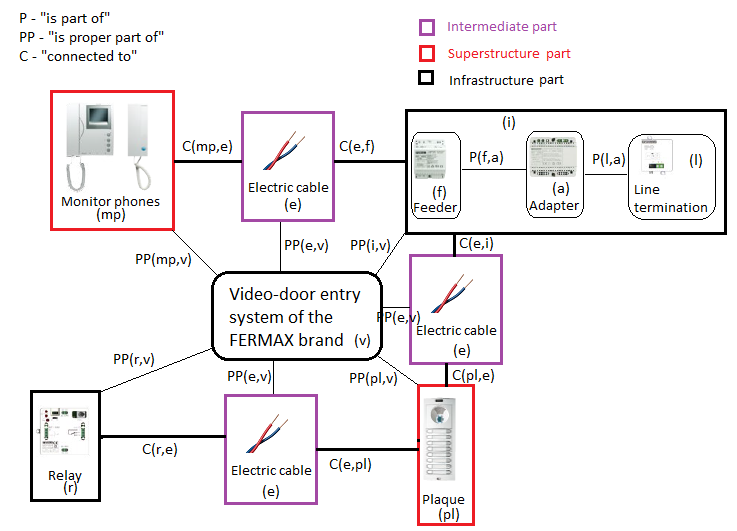
\includegraphics[scale=0.62]{TP1.png}
\caption{A simple example of the use of some mereotopological relationships in a \emph{Whole} as a video-door entry system of the FERMAX brand}\label{TP1}
\end{figure}

Figure \ref{TP1} shows a simple example of some mereotopological relationships in a \emph{Whole} as a video-door entry system of the FERMAX brand. All physical artifacts that conform the configuration of a video-door entry system as a Whole are modeled using P(x,y), PP(x,y) and C(x,y) mereotopological primitives (See tables 1 and 2). In this example only these three primitives are revealed. However, there are examples such as hydraulic systems, heating systems, among others, where more complicated as MSSC(x), SC(x), O(x,y), U(x,y), among others. The above examples, due to their complexity, are being analyzed in depth with the experts in the configuration of electromechanical artifacts, so they are not illustrated in this document.

\begin{table}
% table caption is above the table
\caption{Description of mereotopological primitives for Part-Whole relationships with a heterogeneous structure}
\label{tab:2}       % Give a unique label
% For LaTeX tables use
\begin{tabular}{ll}
\hline\noalign{\smallskip}
Mereotopological description  & Predicate \\
\noalign{\smallskip}\hline\noalign{\smallskip}
${C}(x,y) :={O}(x,y)\vee\exists{z}({O}(z,x)\wedge{B}(z,y)$\\
$\vee{O}(z,y)\wedge{B}(z,x))$ & `\textit{$x$ connected to $y$}' \\
\noalign{\smallskip}\hline\noalign{\smallskip}
${SC}(x) := \forall{y}\forall{z}(\forall{w}({O}(w,x)$ & `\textit{$x$ self-connectedness}' \\
$\leftrightarrow {O}(w,y)\vee{O}(w,z))\rightarrow{C}(y,z)$ &\\
\noalign{\smallskip}\hline\noalign{\smallskip}
${SCW}(x) := \forall{y}\forall{z}(x=y+z\rightarrow{C}(y,z))$ & `\textit{$x$ self-connectedness whole}' \\
\noalign{\smallskip}\hline\noalign{\smallskip}
${ix} :=\sigma{z}{IP}(z,x))$ & `\textit{interior part in $x$}' \\
\noalign{\smallskip}\hline\noalign{\smallskip}
${ex} :={i}(\sim{x})$ & `\textit{exterior part in $x$}' \\
\noalign{\smallskip}\hline\noalign{\smallskip}
${cx} :=\sim ({ex})$ & `\textit{closed part in $x$}' \\
\noalign{\smallskip}\hline\noalign{\smallskip}
${bx} :=\sim ({ix}+{ex})$ & `\textit{limit part in $x$}' \\
\noalign{\smallskip}\hline\noalign{\smallskip}
${SSC}(x) :={SC}(x)\wedge{SC}(ix)$ & `\textit{interior of $x$} \\
 & \textit{self-connectedness}' \\
\noalign{\smallskip}\hline\noalign{\smallskip}
${MSSC}(x):=x=\sigma{y}({P}(x,y)$ & `\textit{$x$ part that is maximally and}\\
$\wedge{SSC}(y))$ & \textit{strongly connected to itself}' \\
\noalign{\smallskip}\hline\noalign{\smallskip}
${MSSC}(x) :=\phi{(x)}\wedge{x}=\sigma{y}({\mathcal{P}}(x,y)$ & `\textit{$x$ part that is maximally and} \\
$\wedge\phi{(x)}\wedge {\mathcal{SSC}}(y))$ & \textit{strongly connected to itself} \\
 & \textit{in relation to any condition $\phi$}' \\
 \noalign{\smallskip}\hline\noalign{\smallskip}
$\sigma{x}(\phi{x}):=\iota{z}\forall{y}({\mathcal{O}}(y,z)$ & '\textit{General sum}\\
$\leftrightarrow\exists{x}(\phi{x}\wedge{\mathcal{O}}(y,x)))$ & \textit{(or sum of $\phi$ers)}' \\
\noalign{\smallskip}\hline\noalign{\smallskip}
${Op}(x) := {x}={ix}$ & `\textit{$x$ open part}' \\
\noalign{\smallskip}\hline\noalign{\smallskip}
${Cl}(x) := {x}={cx}$ & `\textit{$x$ closed part}' \\
\noalign{\smallskip}\hline\noalign{\smallskip}
${Dp}(x,y) :=\phi(y,x)\wedge{P}(y,x)$ & `\textit{$x$ dependent part of $y$}' \\
\noalign{\smallskip}\hline
\end{tabular}
\end{table}

\section{Conclusions and Future Works} \label{C}
This paper describes a new BOM for an ontological model of the industry of manufactured physical artifacts. An abstraction of part-concept of the classical BOM according to the parts that make up a technological artifact (BOP) is presented. In addition, a classification and definition of the structures that are going to describe the BOPs generated is presented. The proposed model is a tool to represent the structure of a technological artifact.
 
As future work, we plan to work on an ontological model on the basis of the new BOM (BOP) described in this work. Besides, we are studying and analyzing a significant sample of mereotopological theories with the aim to identify what relationships of parthood and connectedness types are possible between the parts that make up each one of the structures that describe the BOP. Furthermore, an analysis of the overall relationships by artifacts structure based on their type might help us predict possibles new structures depending on what is type of artifact in correspondence with BOP.
%\vadjust{\vfill\eject}

%%\section*{Acknowledgements}
%%The authors acknowledge the financial support from the FUO-003-16 project by METALUX\footnote{http://metalux.es/} enterprise and University of Oviedo.
%%

%%\section*{References}
\bibliographystyle{ieeetr}
\bibliography{uniovi}



\end{document}